\chapter{Introduction}

To navigate in an unknown environment, a mobile robot needs to build a map of the environment and locate itself in the map at the same time. The process adressing this dual problem is called \gls{SLAM}. In an outdoor environment, this can generally be solved by a GPS that generally allows to get an estimation of the position with a very good accuracy. However, when moving indoor or in places where the GPS data is not available, or not reliable enough, other solutions have to be found. 

Generally, the main problem raised with \gls{SLAM} comes from the measurement errors, due to the sensors noise. Probabilistic models are widely used to reduce these errors and provide satisfying estimations. While this process is generally based on data provided by sensors such as laser scanners, or odometry data, \gls{VSLAM} focuses on the use of camera. 

\begin{figure}[h!]
\begin{center}
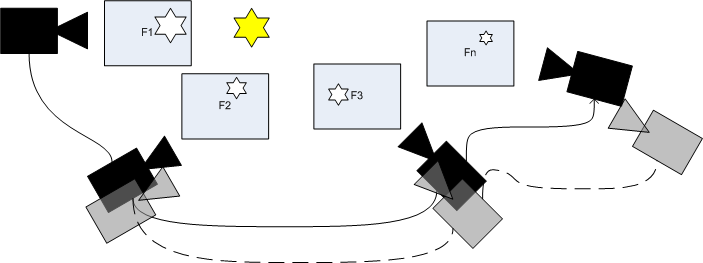
\includegraphics[width=1.0\textwidth]{figures/visual_slam}
\caption{General idea of Visual SLAM - the poses of the camera (hence, the robot for a fixed camera) are determined by the information given by the video. The estimations can lead to a drift with respect to the real trajectory. The uncertainty grows over time.}
\end{center}
\end{figure}

\section{Context}

Currently, most of robotic mapping is performed using sensors that offers only a 2D cross section of the environment around them. One reason is that acquiring high quality 3D data was either very expensive or had hard constraints on the robot movements. However, recently there has been a great interest in processing data acquired using depth measuring sensors due to the availability of cheap and high performance RGB-D cameras. For instance, the Kinect Camera developed by Prime Sense and Microsoft has considerably changed the situation, providing a 3D camera at a very affordable price, with a particular interest for the research projects in robotics.

In the past, to solve the inherent problem of drift and provide a reliable estimation of the camera poses, most of the project were using techniques such as \gls{EKF} or particle filters. More recently, several methods rely on pose graphs to improve the estimation~\cite{Thrun05_GraphSLAM}~\cite{grisetti07rss}~\cite{g2o_2011}~\cite{hogman_2010}. Some projects making use of both RGB-D data and graph optimization~\cite{Henry_RGBD_2010}~\cite{engelhard11euron-workshop} illustrate well the interest of the community for such an approach.

\section{Goals}

This work is done at the \gls{CVAP} at the Royal Institute of Technology, in Stockholm (KTH). The main goal is to build a 3D map from RGB \& depth information provided by a camera. The hardware device used here for the experimentations is the Microsoft Kinect but it could be extended to any RGB-D camera. One objective is to have an overview of the different methods and techniques in order to build a consistent map, so the problems can better be identified and then be individually handled more deeply. Though a \gls{VSLAM} system is intended to be used in real time, some of the processing may be done without focusing on the performance issues in this study. 

The \gls{VSLAM} process can be described as estimating the poses of the camera in order to reconstruct the entire environment while the camera is moving. As the sensor noise lead to deviations in the estimations of each camera poses with respect to the the real motion, the goal is to build a 3D map which is close to the real environment as much as possible.

\clearpage
\section{Thesis outline}

The rest of the document is structured as follows:
\begin{description}
\item[Chapter \ref{chap:background}] presents the background and the underlying concepts that are most commonly used in this area.
\item[Chapter \ref{chap:features}] presents the feature matching and describe how a single 3D transformation can be computed  from a couple of frames by tracking some features.
\item[Chapter \ref{chap:map}] presents how a map can be built, by estimating the camera poses through the use of a pose graph and performing a 3D reconstruction.
\item[Chapter \ref{chap:experiments}] presents the experimentations, the software and how the data was acquired and produced, with examples of maps generated from different datasets.
\item[Chapter \ref{chap:conclusion}] presents the conclusion and the future works with some suggestions of possible improvements.
\end{description}

\chapter{Background}
\label{chap:background}

\section{Microsoft Kinect}

As mentioned in the introduction, the hardware used in this work is the Kinect, a device developed by PrimeSense, initially for the Microsoft Xbox 360 and released in November 2010. It is composed by an RGB camera, 3D depth sensors, a multi-array microphone and a motorized tilt. In this work, only the RGB and depth sensors are used to provide the input data.

\begin{figure}[H]
\centering
\includegraphics[width=0.5\textwidth]{pictures/kinect_sensor}
\caption{the Kinect sensor device (courtesy of Microsoft)}
\end{figure}

Kinect characteristics:
\begin{itemize}
 \item The RGB sensor is a regular camera that streams video with 8 bits for every color channel, giving a 24-bit color depth. Its  color filter array is a Bayer filter mosaic. The color resolution is 640x480 pixels and a maximal frame rate of 30 Hz.
 \item The depth sensing system is composed by an IR emitter projecting structured light, which is captured by the CMOS image sensor, and decoded to produce the depth image of the scene. It has an operation range between 0.7 and 6 meters, although best results are obtained in the range that goes from 1.2 to 3.5 meters. Its data output has 12-bit depth. The depth sensor resolution is 320x240 pixels with a rate of 30Hz.
 \item The field of view is 57\textdegree horizontal 43\textdegree vertical, with a tilt range of $\pm$ 27\textdegree.
\end{itemize}

The drivers used are those developed by OpenNI\footnote{\url{http://www.openni.org/}} (Open Natural Interface). OpenNI is an organization established in November 2010, composed in October 2011 by PrimeSense, Willow Garage, Side-Kick, ASUS, AppSide.

The OpenNI framework offers high level functions which are mainly oriented for the gaming experience, such as gesture recognition and motion tracking. It is an abstraction layer that provides a generic interface to the hardware devices. In the case of the Kinect, one of the main advantages is that the calibration of the RGB sensor with respect to the IR sensor is ensured, so the resulting RGB and depth data are correctly mapped with respect to a unique viewpoint.


\section{Features}

An approach widely used in computer vision, especially in object recognition, is based on the detection of points of interests on object or surfaces. This is done through the extraction of features. In order to track these points of interests during a movement of the camera and/or the robot, a reliable feature has to be invariant to image location, scale and rotation. A few methods are briefly presented here:

\begin{description}
\item[Harris Corner] A corner detector, by Harris and Stephens~\cite{Harris88alvey}
\item[\acrshort{SIFT}]\acrlong{SIFT}, by David Lowe~\cite{lowe_2004_sift} 
\item[\acrshort{SURF}]\acrlong{SURF}~\cite{surf}
\item[\acrshort{NARF}]\acrlong{NARF}~\cite{steder10irosws}
\item[\acrshort{BRIEF}]\acrlong{BRIEF}~\cite{Calonder10-brief}
\end{description}

By feature, two aspects should be distinguised: the detection of a \emph{keypoint} which allows to localize an area of interest, and the \emph{descriptor} of this item, allows to characterize this region. Typically, the detector identifies a region which contains a strong variation of intensity such as an edge or a corner, and its center is designed as a keypoint. The descriptor is generally computed by measuring the main orientations of the surrounding points, leading to a multidimensional \emph{feature vector} which identifies the given keypoint. Given a set of features, a matching can then be performed in order to associate pairs of keypoints, inside an image or between different frames. If we summarize, the mentioned features can be listed as follows :

\begin {table}
 \begin{center}
  \begin{tabular}{c|cc}
  \hline
  Feature & Detector & Descriptor \\
  \hline
  Harris Corner & X & - \\
  SIFT & X & X \\
  SURF & X & X \\
  NARF & X & X \\
  BRIEF & - & X \\
  \hline
  \end{tabular}
 \end{center}
\caption {Characteristics of the features}
\end{table}

\subsection{Harris Corner}

Known as the Harris corner operator, this is one of the earliest detector, as it was proposed in 1988 by Harris and Stephens~\cite{Harris88alvey}. The  notion of corner should be taken in a wide sense as it allows to detect not only corners, but edges and more generally, keypoints. It is done by computing the second moment matrix. It is an important reference to mention as it has been used as the basis for further works and improvements leading to more recent methods. One of the main limitation with the Harris operator concerns the scale invariance.

\subsection{SIFT feature}

\glsreset{SIFT}
The \gls{SIFT} is a method presented by David Lowe~\cite{lowe_2004_sift}, now widely used in robotics and computer vision.
This is a method to detect distinctive, invariant image feature points, which easily can be matched between images to perform tasks such as object detection and recognition, or to compute geometrical transformations between images.

The main idea of the \gls{SIFT} method is to define a cascade of operations following an increasing complexity, so that the most expensive operations are only performed to the most probable candidates.
\begin{enumerate}
\item The first step relies on a pyramid of \gls{DoG} in order to be invariant to scale and orientation.
\item From this, stable keypoints are determined with a more accurate model.
\item The image gradient directions is then used to assign one or more orientations to the keypoints.
\item The local image gradients are then transformed to be stable against distortion and changes in illumination.
\end{enumerate}

\clearpage
\paragraph{\emph{Detector}}

Most of these concepts concerning the study of the scale space are based on the works of Lindeberg~\cite{Lindeberg_1994}. The general concept is shown in \ref{fig:sift_dog}. First, the scale space is defined as the convolution of an image~$I$ with a Gaussian~$G$ with variance~$\sigma$.

\[ L(x,y,\sigma) = G(x,y,\sigma) * I(x,y) \]

where

\[ G(x,y,\sigma) = \frac{1}{2\pi\sigma^2}e^{-{(x^2+y^2)/2\sigma^2}} \]


The \gls{DoG} is the difference between two layers in scale space along the $\sigma$ axis:

\[
\begin{array}{rcl}
D(x,y,\sigma) & = & (G(x,y, k\sigma) - G(x,y,\sigma)) * I(x,y) \\
 & = & L(x,y,k\sigma) - L(x,y,\sigma)
\end{array}
\] 

This provides a close approximation to the scale-normalized Laplacian of Gaussian $\sigma^2\nabla^2G$, as shown by Lindeberg ~\cite{Lindeberg_1994}:

\[ \sigma\nabla^2G = \frac{\partial G}{\partial \sigma} \approx \frac{G(x,y,k\sigma)-G(x,y,\sigma)}{k\sigma - \sigma} \]

and therefore:

\[ G(x,y,k\sigma) - G(x,y,\sigma) \approx (k-1)\sigma^2\nabla^2G \]

The $\sigma^2$ factor allows the scale invariance. Then, the localization of the keypoints is done by finding the extrema in the \gls{DoG}, which approximates the Laplacian~$\sigma^2\nabla^2G$. Lowe shows that the remaining factor $(k-1)$ does not influence the location. 

\begin{figure}[h]
\centering
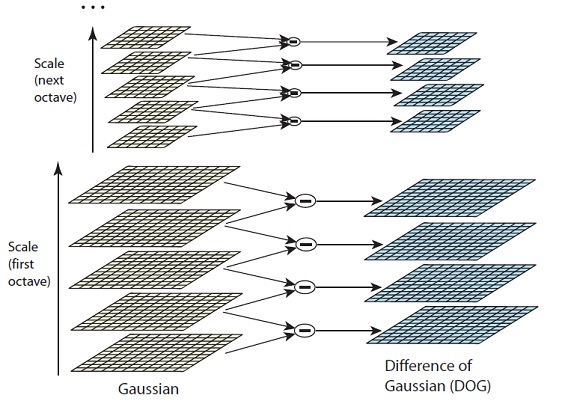
\includegraphics[width=0.8\textwidth]{figures/sift_dog}
\caption{Difference of Gaussians at different scales (courtesy of David Lowe) - For each octave of the scale space, the image is convolved with a Gaussian, which variance~$\sigma$ is multiplied each time by a constant factor. Two consecutive results are substracted to give the DoG which approximates the Laplacian of Gaussian. After each octave, the image is downsampled by two, and the process is repeated doubling the variance~$\sigma$. The initial value of~$\sigma$ can be changed accordingly to the type of application. }
\label{fig:sift_dog}
\end{figure}

\paragraph{\emph{Descriptor}}

In order to provide a good basis for the matching, the descriptor has to be highly distinctive and invariant to remaining variations such as change in illumination or 3D viewpoint. The \gls{SIFT} descriptor is based on a \gls{HoG} around the keypoint. It is stored as a 128 dimensional feature vector (4x4 descriptor with 8 orientation bins). The figure \ref{fig:sift_descriptor} illustrates this concept with a smaller 2x2 descriptor.

\begin{figure}[h]
\centering
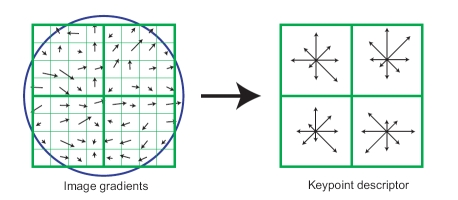
\includegraphics[width=0.8\textwidth]{figures/sift_descriptor}
\caption{SIFT descriptor (courtesy of David Lowe) - illustration of how the gradient directions are accumulated into orientation histograms around the center of the region defined by the keypoint. The gradients are first weighted by a Gaussian window represented by the circle. From the 8x8 sample, a 2x2 descriptor is computed this way, where each bin covers a 4x4 subregion.}
\label{fig:sift_descriptor}
\end{figure}

\clearpage
\paragraph{\emph{Matching}}

Once the keypoints are found and the descriptors computed, the next step is to be able to perform fast searches on the features in order to identify candidate matching. Refer to the method described in~\cite{lowe_2004_sift} for further details.

\begin{figure}[h]
\centering
\includegraphics[width=0.8\textwidth]{pictures/sift_matches_robhess}
\caption{SIFT features matched between the two images}
\end{figure}

For this work, we use the \gls{SIFT} library developed by Rob Hess~\cite{hess_sift}. Additionally to the feature extraction, this library also provides a function to perform the initial matching through a kd-tree. There are also other functions such as a extendable function that can be used to compute geometrical transformations with \gls{RANSAC} (method described in ~\ref{sub:ransac}) but the given functions are only working for 2D operations and will not be used.

\subsection{SURF feature}

\glsreset{SURF}
The \gls{SURF} is a robust image detector \& descriptor~\cite{surf}, that can be used in computer vision tasks like object recognition or 3D reconstruction. It is partly inspired by the \gls{SIFT} descriptor, both are using local gradient histograms. The main difference concerns the performance, lowering the computational time through an efficient use of integral images for the image convolutions, hessian matrix-based detector (optimized through approximations of the second order Gaussian partial derivatives), and sums of approximated 2D Haar wavelet responses for the descriptor. The standard version of \gls{SURF} is several times faster than \gls{SIFT} and claimed by its authors to be more robust against different image transformations than \gls{SIFT}.

\begin{figure}[H]
\centering
 \begin{tabular}{cc}
 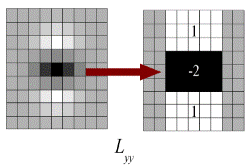
\includegraphics[width=0.4\textwidth]{figures/surf_lyy} &
 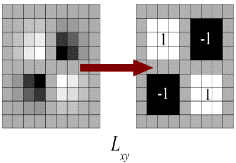
\includegraphics[width=0.4\textwidth]{figures/surf_lxy}
 \end{tabular}
\caption{SURF detector relies on approximation of the Gaussian second order derivatives}
\end{figure}

\begin{figure}[H]
\centering
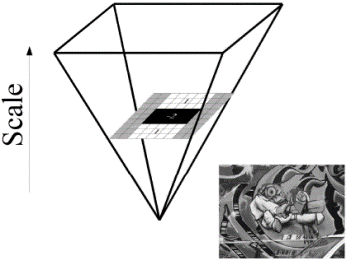
\includegraphics[width=0.4\textwidth]{figures/surf_scale}
\caption{SURF scale space is built by changing the filter size}
\end{figure}

\begin{figure}[H]
\centering
 \begin{tabular}{cc}
 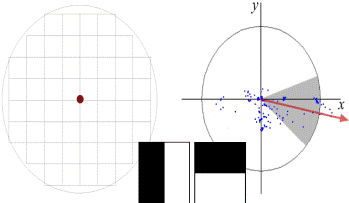
\includegraphics[width=0.4\textwidth]{figures/surf_orientation} &
 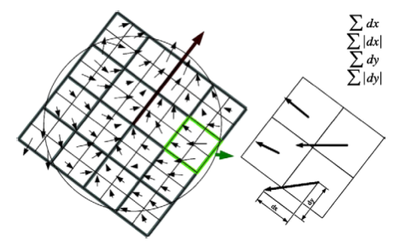
\includegraphics[width=0.4\textwidth]{figures/surf_descriptor}
\end{tabular}
\caption{SURF keypoint orientation is found by summing up the response of Haar wavelets with a sliding window of 60 degrees. The descriptor is finally computed by splitting the region around the keypoint into 4x4 subregions and computing Haar wavelet responses weighted with a Gaussian kernel}
\end{figure}

\subsection{NARF feature}

\glsreset{NARF}
The \gls{NARF} is presented by Bastian Steder in~\cite{steder10irosws}. It is meant to be used on single range scan obtained with 3D laser range finders or stereo camera. This work is part of the \gls{PCL}~\cite{Rusu_ICRA2011_PCL} which is itself a component of the \gls{ROS}. Its detector looks for stable areas with significant change in vicinity, that can be identified from different viewpoints. The descriptor characterizes the area around the keypoint by calculating a normal aligned range value patch and finding the dominant orientation of the neighbouring pixels.

\begin{figure}[H]
\centering
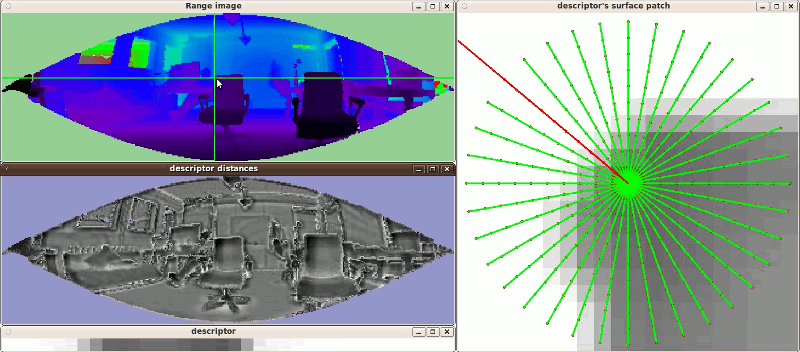
\includegraphics[width=0.8\textwidth]{figures/narf_descriptor_visualization}
\caption{NARF feature (courtesy of Bastian Steder) - from the range image a descriptor is computed in the given keypoint localized by the position of the green cross. The right figure shows the surface patch containing the corner of the armchair and the dominant orientation pointed by the red arrow. Each component of the descriptor is associated to a direction given by one of the green beams. The bottom left picture shows the values of this descriptor. The middle left figure shows the distance to this descriptor for any point in the scene, and therefore their similarity with the current keypoint. The darkest areas are the closest, identifying the areas which are the most similar to the left corner of the armchair.}
\end{figure}

\begin{figure}[H]
\centering
\includegraphics[width=0.5\textwidth]{pictures/narf1}
\caption{Example of NARF keypoints computed on a desk}
\end{figure}

\subsection{BRIEF feature}

\glsreset{BRIEF}
The \gls{BRIEF} presented in~\cite{Calonder10-brief} is an efficient alternative for the descriptor, based on binary strings computed directly from image patches and using Hamming distance instead of the $L_2$ norm commonly used on higher dimension descriptors. As the binary comparison can be performed very efficiently, the matching between several candidates can be done much faster. The use of a \gls{BRIEF} descriptor supposes the keypoints are already known, this can be done with a detector such as \gls{SIFT} or \gls{SURF}. A deeper study is available in the PhD thesis of Calonder~\cite{Calonder10_PhD}, which is the main author of the \gls{BRIEF} features. This document presents comparative evaluation of \gls{BRIEF}, \gls{SIFT} and \gls{SURF}.

\section{Computing a transformation}

Once the features have been computed, the question is to be able to track them during the movement of the camera. This is done by associating them between different frames. Here we only consider the matching for a couple of frames, the process can then be repeated on the whole sequence of frames. To associate several pairs of features is not straightforward, as the descriptors are not exactly the same between two different frames, first as a consequence of the movement of the camera and also because of the noise. The best matching then consists in finding the correct associations with a good belief. Most of the algorithms work with different steps, first from a scarse level where the hypothesis is wide, which is then refined to eliminate the most obvious mismatches. The matches that fit to the model are called the \emph{inliers}, while the remaining matches errated are called the \emph{outliers}.

\subsection{RANSAC}
\label{sub:ransac}

\glsreset{RANSAC}
The \gls{RANSAC} is an iterative method, widely known in the computer vision, to estimate the parameters of a transformation given a dataset. It was published in 1981 \cite{FischlerB81}. With a classic least square approach, the parameters which satisfy the whole dataset can be found, but this is not generally the best one when there are some noisy points. Here, the idea is to find the parameters which are valid for most of the points, by discarding the noisy points from the consensus. For each iteration, a very small number of samples are \emph{randomly} selected to define a model, representing one hypothesis. This model is then evaluated for the whole dataset. This is repeated several times by choosing new samples for each iteration and keeping the best transformation found. After running this for a fixed number of steps, the algorithm is guaranteed to converge to a better transformation (with a lower error), but it does not necessarily find the best one, as all the possibilities have not been tested. 

\begin{algorithm}
\caption{General RANSAC}\label{alg:generic_ransac}
\begin{algorithmic}
\REQUIRE Dataset of points
\STATE Define the number of iterations $N$;
\FOR{$iteration = 1$ to $N$}
 \STATE $samples \gets$ Pickup k points randomly;
 \STATE Compute $currentModel$ from $samples$ (base hypothesis);
 \STATE $inliers \gets \emptyset$;
 \FORALL{points}
  \STATE Evaluate $currentModel$ for the point and compute its error;
  \IF{$error < threshold$}
   \STATE $inliers \gets inliers + point$;
  \ENDIF
 \ENDFOR
 \STATE Count number of inliers and compute mean error;
 \IF{$currentModel$ is valid}
  \STATE Recompute $currentModel$ from $inliers$;
  \IF{$currentModel$ better than $bestModel$}
   \STATE $bestModel \gets currentModel$;
   \STATE $bestInliers \gets inliers$;
  \ENDIF
 \ENDIF
\ENDFOR
\RETURN $bestModel$, $bestInliers$;
\end{algorithmic}
\end{algorithm}

\begin{figure}
\centering$
\begin{array}{|c|c|c|}
\hline
\subfloat[]{\label{fig:exransac1} \includegraphics[width=0.3\textwidth]{figures/ransac1}} &
\subfloat[]{\label{fig:exransac2} 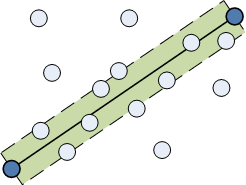
\includegraphics[width=0.3\textwidth]{figures/ransac2}} & 
\subfloat[]{\label{fig:exransac3} 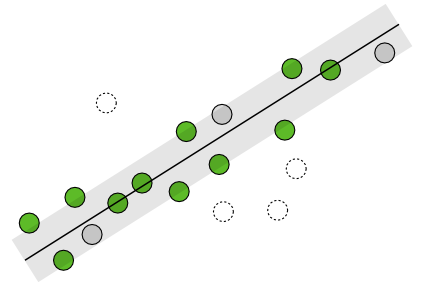
\includegraphics[width=0.3\textwidth]{figures/ransac3}} \\
\hline
\end{array}$
\caption{Illustration of a RANSAC iteration, for a 2D dataset. \protect\subref{fig:exransac1}~First, k items are chosen randomly among the set (here k=2). \protect\subref{fig:exransac2}~From these points, a model is defined. Here, a line is drawn between the 2 chosen points, with an area of validity defined by a given threshold. \protect\subref{fig:exransac3}~The model is then evaluated by measuring the error for each point, here by computing the distance to the line. This separates the dataset into two subsets: the inliers, in green (fitting to the model) and the outliers, in red (ignored). The ratio of inliers relatively to the total number of items can give a numerical evaluation of the model ("goodness"). The initial model is generally recomputed taken all the inliers into account.}
\end{figure}

The main difficulty with the \gls{RANSAC} algorithm is to define the number of iterations and the thresholds.
For the number of iterations, it is possible to define the ideal value according to a desired probability. Considering a sample of $k$ points, randomly chosen, if $p$ denotes the probability that at least one of the sample set does not include an outlier, $u$ the probability of observing an inlier, we have then:

\[
1-p = (1-u^k)^N
\]

It can be more convenient to define $v=1-u$ as the probability of observing an outlier. From this, we can obtain the required number of iterations:

\[
N = \frac{log(1-p)}{log(1-(1-v)^k)}
\]

For the threshold, it depends of the problem and the application, generally this is done empirically with the standard method. There are many variants of the \gls{RANSAC} that try to overcome this problem, such as the MLESAC method \cite{TorrZ00} using M-estimators in order to find the good parameters in a robust way.


\subsection{ICP}

\glsreset{ICP}
The \gls{ICP} is an algorithm presented by Zhang~\cite{zhang_92_icp}.
It iteratively revises the rigid transformation needed to minimize the distance between the points of two raw scans. Considering two sets of points $(p_{i}, q_{i})$, the scope is to find the optimal transformation, composed by a translation $t$ and a rotation $R$, to align the source set $(p_{i})$ to the target $(q_{i})$. The problem can be formulated as minimizing the squared distance between each neighboring pairs:

\[min \sum_{i}{||(Rp_{i}+t)-q_{i}||}^2\]

As any gradient descent method, the \gls{ICP} is applicable when we have in advance an relatively good initial guess. Otherwise, it is likely to be trapped into a local minimum. One possibility, as done by Henry~\cite{Henry_RGBD_2010}, is to run \gls{RANSAC} first to determine a good approximation of the rigid transformation, and use it as the first guess for the \gls{ICP} procedure.

\clearpage
\section{General concepts for SLAM}

As described in the introduction, the \gls{SLAM} problem can be defined as looking for the best estimation of the robot/camera poses, by reducing the uncertainty due to the noise affecting the measurements. This leads to use the probabilistic approach such as Expectation Maximization techniques widely described in~\cite{Thrun_2005}. The underlying idea is to compute a most likely map, and every time the estimation of the robot pose is known with more accuracy, the previously computed map is updated and the process is repeated. The momentary estimation of the position, or $belief$, is represented by a probability density function. 

By denoting $x_t$ the state of the robot at time t (representing the robot's motion variables such as the poses), $z_t$ a measurement (for example camera images or laser range scans), and $u_t$ the control data (denoting the changes of state), the belief over the state variable $x_t$ is given by:

\[bel(x_t) = p(x_t | z_{1:t}, u_{1:t})\]

This posterior is the probability distribution over the state $x_t$ at time $t$, conditioned on all past measurements $z_{1:t}$ and all past controls $u_{1:t}$.

In the case of \gls{VSLAM}, we consider the video sequence as a collection of frames, defined by a flow of RGB \& Depth data coming from the Kinect. Here we use exclusively the video, and therefore each measurement $z_t$ is a couple of RGB \& Depth frame at time $t$ . The number of frames then depends on the length of the sequence and the effective frame rate, which is bounded by the maximum rate of the Kinect which is 30Hz.


\subsection{Filtering vs Smoothing}

To solve the \gls{SLAM} problem, the literature presents different approaches that can be classified either as filtering or smoothing. Filtering approaches model the problem as an on-line state estimation where the state of the system consists in the current robot position and the map. The estimate is augmented and refined by incorporating the new measurements as they become available.
The most common techniques are the \glsreset{EKF}\gls{EKF} and the particle filters. To highlight their incremental nature, the filtering approaches are usually referred to as on-line \gls{SLAM} methods.
The major drawback of these techniques is the computational cost. As the robot moves, the quantity of data to be handled becomes bigger.

Conversely, smoothing approaches estimate the full trajectory of the robot from the full set of measurements. These approaches address the so-called full \gls{SLAM} problem, and they typically rely on least-square error minimization techniques.

Recently, the performance of the graph optimization has been dramatically improved. In this work, we will therefore study the results that can be obtained from a graph-based approach. In contrast to the online techniques, the pose graph is said to be offline or a "lazy" technique as the optimization processing triggered by specific constraints.

\subsection{Pose Graph}

The \gls{SLAM} problem can be defined as a least squares optimization of an error function described by a graph. Such a graph is called a pose graph. In a general way, the problem can be formulated by a graph where the nodes (or vertices) represent a state variable describing the poses of the cameras, and the edges would represent the related constraints between the observations connecting a pair of nodes. Not only the graph representation gives a quite intuitive representation of the problem, but the graph model is also the base for the mathematical optimization, which purpose is to find the most-likely configuration of the nodes.

Here we present different approaches:

\begin{description}
\item[GraphSLAM] Probabilistic robotics~\cite{Thrun_2005} represents beliefs through conditional probability distributions. A belief distribution assigns a probability (or density value) to each possible hypothesis with regards to the true state. Belief distributions are posterior probabilities over state variables conditioned on the available data. The idea behind GraphSLAM~\cite{Thrun05_GraphSLAM} is to represent constraints, defined by the likelihoods of the measurements and motions models, in a graph. The computation of the posterior map is achevied by solving the optimization problem, taking all the constraints into account.
\item[TORO] a Tree-based netwORk Optimizer ~\cite{grisetti07rss}. A least square error minimization technique based on a network of relations is applied to find maximum likelihood (ML) maps. This is done by using a variant of gradient descent to minimize the error, by taking steps proportional to the negative of the gradient (or its approximation). It is used in the 3D dense modeling project led by Henry~\cite{Henry_RGBD_2010}.
\item[HOG-Man] Hierarchical Optimizations on Manifolds for Online 2D and 3D mapping~\cite{hogman_2010}: this approach considers different levels. Solving the problem on lower levels affects only partially the upper levels. Well adapted for large maps. It is used in the RGBD-6D-SLAM~project~\cite{engelhard11euron-workshop}.
\item[$g^2o$] General Framework for Graph Optimization~\cite{g2o_2011}, by the same authors of HOG-Man~\cite{hogman_2010}. $g^2o$ is a framework which gives the possibility to redefine very precisely the error function to be minized and how the solver should perform it. Some classes are provided for the most common problems such as 2D/3D \gls{SLAM} or Bundle Adjustement. The HOG-Man concepts are likely to be integrated in $g^2o$. This is the method chosen to solve the graph problem in this work.
\end{description}

\subsection{Loop closure}

In order to minimize the error, the graph optimization relies on constraints between the nodes. One interesting event occurs when the robot moves back to a position already visited in the past. This is refered as the \emph{loop closure} detection. To illustrate this, let us take an example. Imagine you are visiting a new city and you have just arrived at your hotel. Without taking a map, you would like to explore the neighbourhoods but you still want to keep track of the path you follow with a scarse definition of the environment (mentally, or drawing it on a paper). After walking for a while around a few blocks, you don't know any longer exactly where you are. However, by following a circular path, or a squared path considering standard blocks, you will probably pass again by places you have already visited. By recognizing these places, you are now able to estimate more precisely the path you actually followed and correct the related map.

The loop closure detection relies basically on this idea. Without making an assumption on the path followed by the robot, and simply by keeping the history of the past frames, it is possible to check if the current frame matches with some of the previous ones. If the current observation is close to a previous one, a transformation can be computed between these frames and a new constraint can be inserted from it. This can be repeated several times. With these new constraints, the cumulated error of the graph can then be considerably reduced. Theorically, all the poses could be linked together this way. 

\begin{figure}[H]
\centering$
\begin{array}{cc}
\subfloat[]{\label{fig:lc1} 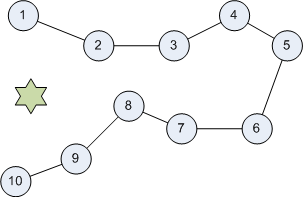
\includegraphics[width=0.4\textwidth]{figures/graph_lc1}} &
\subfloat[]{\label{fig:lc2} 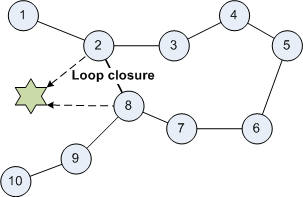
\includegraphics[width=0.4\textwidth]{figures/graph_lc2}}
\end{array}$
\caption{Loop closure detection. \protect\subref{fig:lc1}~The poses are linked together by standard edges, each one represents a transformation. \protect\subref{fig:lc2}~The observation of a common point of interest already seen in the past, if significant, can trigger the creation of a new link between two poses that were previously separated in the whole sequence.}
\end{figure}

\begin{figure}[H]
\centering
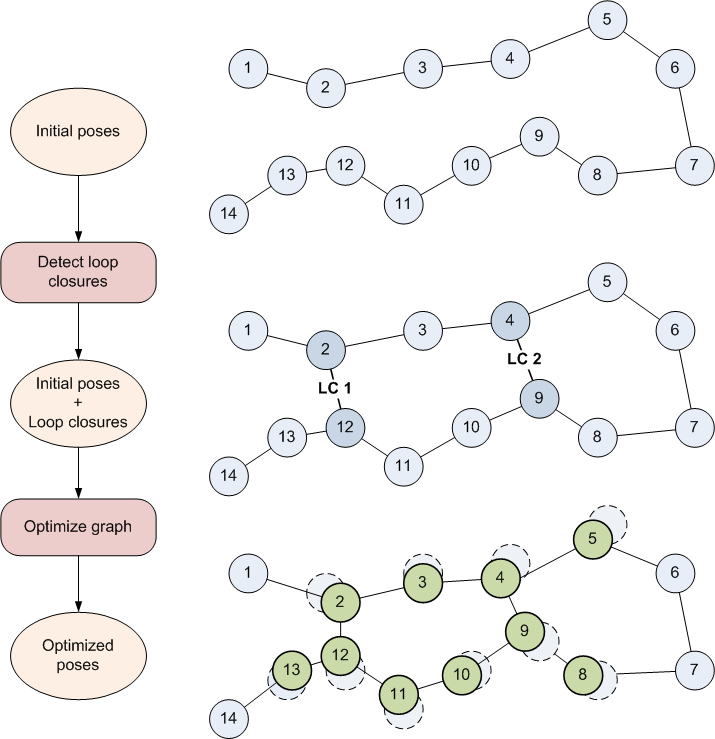
\includegraphics[width=1\textwidth]{figures/graph_overview}
\caption{Overview of the graph optimization procedure. The detection of loop closures leads to the insertion of new edges. The optimization of the graph consists in finding the optimal configuration of vertices to respect all the given constraints.}
\end{figure}

\clearpage
\section{Summary}

This chapter gives an overview of some of the main concepts used for \gls{SLAM} and more specifically \gls{VSLAM}, defining the main lines of a possible approach to solve the problem. The features allow to track some points of interest and can be used to evaluate a single move from a couple of frames. By combining them together an estimation of the trajectory of the camera could be estimated. With the use of a pose graph, and after detecting loop closures, the graph could be optimized in order to reduce the global drift error. From the corrected camera poses, a map can then be built. 

While the performance is not the main issue of this work, it is still possible to make a distinction between the operations that can be performed \emph{online} (while the robot is moving) and the operations done \emph{offline} (after a given sequence of moves). While the \gls{SLAM} adresses both Localization and Mapping, the solution based on the graph implies the detection of loop closures to give a correct result. Therefore the dual problem of building the map and localizating the robot at the same time is more likely to be done \emph{offline}. This is one of the main constraint resulting of this approach. However, once the map is built, the single operation of localization could be done on the basis of the relevant features that have been used during the initial \gls{SLAM} operation. This kind of approach could allow the robot to build a map as a first step, only for this purpose. Once the map is built, the localization and further operations could be done but this mainly depends on the tasks the robot has to fulfill.

\chapter{Feature matching}
\label{chap:features}

\section{Feature extraction}

The first question is the choice of the features. In the context of \gls{VSLAM}, the goal is to track some keypoints precisely in order to compute the motion of the camera from the keypoint coordinates. For this, in addition to the scale and rotation invariance, one important condition that can be easily verified is to be stable if the camera does not move. 

Here we first tested the \gls{SIFT} features~\cite{lowe_2004_sift} with the library developed by Rob Hess~\cite{hess_sift}, and the \gls{NARF} descriptor~\cite{steder10irosws} provided by the \gls{PCL}. One important difference is that the \gls{SIFT} feature is computed from the RGB data in 2D, while the \gls{NARF} keypoints are computed from the 3D point cloud, involving both RGB and Depth data.
The \gls{NARF} keypoints showed to be unstable, as shown below while the camera was not moving.

%\begin{figure}[h]
%\centering$
% \begin{array}{cc}
% \includegraphics[width=0.5\textwidth]{pictures/narf1_a} &
% \includegraphics[width=0.5\textwidth]{pictures/narf2_a}
% \end{array}$
%\caption{Example of NARF keypoints computed from two consecutive frames without moving the camera. The marks show some keypoints that differs (new or moved).}
%\end{figure}

These variations could be explained by the noise of the depth data of the Kinect, affecting the \gls{NARF} detector. It is possible that some tuning would help to get more stable results, but the \gls{NARF} was mainly designed for range scans such as laser range finders or stereo cameras which are generally more accurate and probably less sensible to noise than the Kinect sensor. For this reason, we prefered to work with the 2D image, using \gls{SIFT} feature~\cite{lowe_2004_sift} which is widely used in the community and is known to be distinctive. In order to keep only features that are interesting for the next steps of the processing, the features are removed if the depth data on this point is not available (occlusion) or if the depth data is outside a fixed range of depth distance. Here a maximum range of 5 meters is used.

Practically, there are many parameters to define how the \gls{SIFT} features are extracted. This will mainly affect the number of features and the computational time. In particular, it concerns how many scales ($k$) are computed for each octave and the variance ($\sigma$) of the Gaussian. Here, the default values of the \gls{SIFT} library~\cite{hess_sift} are used, refering themselves to the standard values recommanded by David Lowe ($k=3$, $\sigma=1.6$). Refer to the method~\cite{lowe_2004_sift} for the description of these parameters.

\section{Comparison of SIFT/SURF features}
After testing and getting good results with the \gls{SIFT} feature, the same experiments were repeated, using the \gls{SURF} features. The implementation of OpenCV was used. We noticed a considerable gain in performance for a similar number of features. Globally, for a scene requiring about 1000ms with \gls{SIFT}, the extraction of the \gls{SURF} feature takes about 250ms, meaning that the time is reduced by a factor of 4 which is considerable.
However, both algorithms have various parameters that will result in more or less features at the cost of computational time. These parameters are for example the number of octaves (see figure \ref{fig:sift_dog}), and the Hessian threshold for SURF (only features with Hessian larger than that are extracted). In order to compare both methods, we first tried to find a configuration of parameters giving similar number of features, using a dataset of 6474 frames described in chapter \ref{chap:experiments}. For an image of 640x480 pixels, the number of octaves set in the SIFT Library is 6. By setting the same number of octaves at 6 and a Hessian threshold of 300 for \gls{SURF}, we get a very close number of features. Then, we compare with the default settings which implies a number of octaves of 3 and a Hessian threshold of 500. The results are summarized in the table \ref{tab:stats_features}.

\begin{table}[h]
 \begin{center}
 \begin{tabular}{r|ccc}
 & Nb Features & Time & Time by Feature \\
 &  & (in ms) & (in ms) \\
 \hline
 SIFT 6 & 745 & 894 & 1.407\\
 SURF 6/300 & 711  & 345  & 0.582 \\
 SURF 3/500 & 384 & 178 & 0.586 \\
 \end{tabular}
\caption{Comparison of SIFT and SURF features, averaged for 6474 frames. For a similar number of features, SURF is almost 3 times faster than SIFT. For half number of features, there is a gain of factor 5. For various settings of SURF, the time by feature remains constant.}
\label{tab:stats_features}
\end{center}
\end{table}

\begin{figure}[H]
\begin{center}
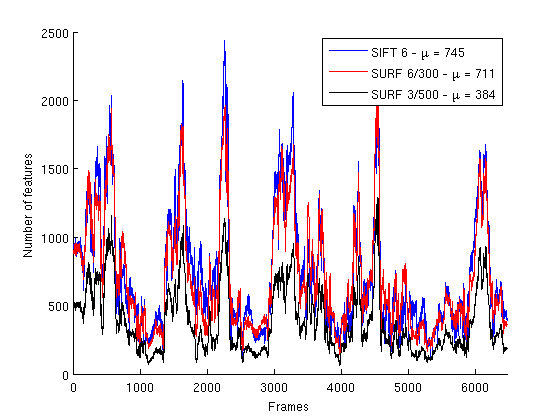
\includegraphics[width=0.7\textwidth]{figures/stats_features_nb}
\caption{Comparison of SIFT and SURF - number of features: default SIFT and SURF 6/300 are similar, while SURF 3/500 give half number of features.}
\end{center}
\end{figure}

\begin{figure}[H]
\begin{center}
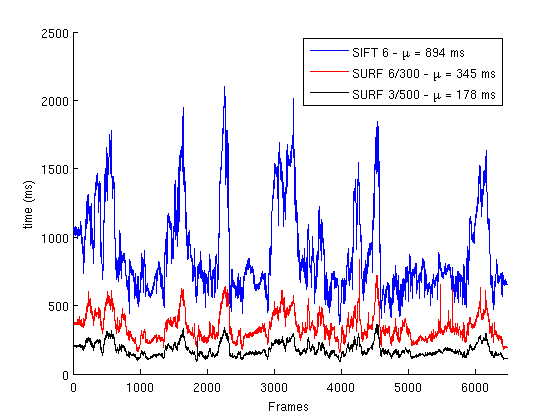
\includegraphics[width=0.7\textwidth]{figures/stats_features_time}
\caption{Comparison of SIFT and SURF - time for computing features: SURF is about 2.6 times faster than SIFT for a similar number of features. For different SURF parameters, the time is linearly proportional to the number of features (x2 faster for x2 less features).}
\end{center}
\end{figure}

\begin{figure}[H]
\begin{center}
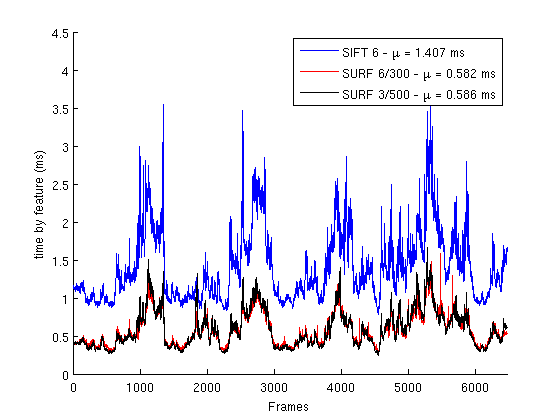
\includegraphics[width=0.7\textwidth]{figures/stats_features_tbf}
\caption{Comparison of SIFT and SURF - average time by feature: SURF is fastest and it does not depend on the given parameters.}
\end{center}
\end{figure}

\section{Initial Matching}

Now that the features can be computed, it is possible to perform some feature matching between a couple of frames, to get the initial matches. This is done through a nearest neighbour search, using the Euclidean distance of these features.  
The SIFT Library~\cite{hess_sift} proposes an implementation of the Best Bin Search described by Lowe~\cite{lowe_2004_sift}, based on kd-tree. For each feature in the target frame, the 2 nearest neighbours are searched in the source frame. If these neighbours are close enough (with respect to a fixed threshold), then the result is considered to be valid. This first search is done on the 2D features. To increase robustness, matches are rejected for those keypoints for which the ratio of the nearest neighbour distance to the second nearest neighbour distance is greater than a given threshold, set to 0.5 here. After this, the depth information is used to keep the features that are close enough, as the accuracy of the depth information is not considered reliable enough above a given range (around 5-6 meters).

\begin{figure}[H]
\centering
\includegraphics[width=0.6\textwidth]{pictures/sift_matching_init}
\caption{Initial matching of SIFT features}
\end{figure}

\section{Estimation of the 3D transformation}

From the matching pairs, it is possible to find a rigid transformation binding the two sets of points, ie the operation that transforms each feature point of a source frame to the corresponding point in the target frame. In our case, this transformation is a perspective projection for 6 degrees of freedom, composed by a rotation matrix and a translation vector in 3 dimensions. This transformation can be written by using a 4x4  matrix and homogeneous coordinates. We can then project a point P where $P = (x,y,z,1)^T$ simply by applying this transformation matrix to the point:

\[
P' = T_{transformation} \: P
\]

The points defined by the initial matching pairs need to be converted in 3 dimensions. For this, we need to define a proper coordinate system. To make the next steps easier (graph optimization and scence reconstruction) and avoid further conversions, we keep the same coordinate system for all the work, defined as follows:

\[
\left\{\begin{array}{l}
x: depth,\:positive\:forward\\
y: height,\:positive\:upwards\\
z: width,\:positive\:to\:the\:right\\
\end{array}
\right.
\]

\begin{figure}[H]
\centering
\includegraphics[width=0.8\textwidth]{figures/coordinates}
\caption{The two different coordinate systems, from the "screen" (as seen by the sensors RGB-D) to the 3D scene in the real world.}
\end{figure}

From the depth value (given in mm by OpenNI) and the screen coordinates (with RGB color and a resolution of 640x480 pixels), it is possible to compute the points coordinates in 3D. Let (u,v) be the point coordinates in pixels, we have then:

\[
P(x,y,z)\left\{
\begin{array}{l}
x = depth \\
y = -(v - 480/2) * depth / focal\_length \\
z = (u - 640/2) * depth / focal\_length \\
\end{array}
\right.
\]

\paragraph{}
Considering the initial matches, the next step is then to find a transformation matrix that fits best to these points. Ideally we could simply compute a transformation by a least square method for all these points, each matching pair defining an equation. The minimum number of pairs required for this would be three, and the more points, the better defined the system would be. However, due to the uncertainty like the noise coming from the sensors, a single point which location is uncorrectly estimated could lead to a big error in the final transformation. Therefore, a better transformation can be found iteratively with the \gls{RANSAC} method presented in the background~(\ref{sub:ransac}). In this context, we can precise the algorithm:

\begin{algorithm}[H]
\caption{Find the 3D transformation with RANSAC}
\begin{algorithmic}
\REQUIRE initial pairs of 3D points (origin, destination)
\STATE Define the number of iterations $N$;
\FOR{$iteration=1$ to $N$}
 \STATE $samples \gets$ pickup randomly k pairs (origin, destination);
 \STATE Compute $currentTransform$ from $samples$;
 \STATE $inliers \gets \emptyset$;
 \FORALL{pairs of points}
  \STATE $projected_i \gets$ projectPoint($origin_i$, $currentTransform$);
  \STATE $error \gets$ computeDistance($projected_i - destination_i$);
  \IF{$error$ < $threshold$}
   \STATE{$inliers \gets inliers + pair_i$};
  \ENDIF
 \ENDFOR
 \STATE Count number of inliers and compute mean error;
 \IF{$currentTransform$ is valid}
  \STATE Recompute $currentTransform$ from $inliers$;
  \IF{$currentTransform$ better than $bestTransform$}
   \STATE $bestTransform \gets currentTransform$;
   \STATE $bestInliers \gets inliers$;
  \ENDIF
 \ENDIF
\ENDFOR
\RETURN $bestTransform$, $bestInliers$;
\end{algorithmic}
\end{algorithm}

As presented in the background, it is possible to estimate the optimal value of N to fulfill a target probability of having a desired number/ratio of inliers (or outliers). In this work we use a fixed value given by parameter of N=20. A deeper study of the \gls{RANSAC} step could lead to tune more accurately this parameter. Generally, if the quantity of features is high, the probability of having an outlier is very low at this point, as most of the mismatches have already been excluded by the initial matching round.

%If we define that the mean number of features is 500 with 10 outliers (after different experiments) then we have:
%\[
%v=10/500=1/50
%N = \frac{log(1-p)}{log(1-(1-v)^k)} = \frac{log(1-0.99)}{log(1-(1-\frac{1}{50})^3)} = 
%\]

To compute a transformation (an hypothesis), only the k samples from the initial matches are used each time. The 3D points are converted to homogeneous coordinates and the transformation is given by solving the corresponding equation from the known constraints which are defined by the chosen points. This is can be done through a \gls{SVD} of the covariance data. To do this, we use the minimal number of points to solve this equation, k=3.

To evaluate a transformation, each sample taken from the initial matches (source) is then projected according to this transformation. A 3D vector is computed from the difference between the projected point and the real point taken from the matching point (destination). The error is the norm of this vector.

\section{Analysis}

Some preliminar experiments were conducted to determine how to find a satisfying transformation between a couple of frames. In the context of \gls{VSLAM}, the local move between two frames should be generally low if we consider a limited move of the camera. The larger the move, the more difficult it becomes. To do this, a program was written to perform the feature extraction with the initial matching and the RANSAC iterations, taking a couple of RGB-D frames as an input.

\begin{figure}[H]
\centering$
 \begin{array}{cc}
 \subfloat[]{\label{fig:sift_match_1} \includegraphics[width=0.5\textwidth]{pictures/sift_matching_init}} &
 \subfloat[]{\label{fig:sift_match_2} \includegraphics[width=0.5\textwidth]{pictures/sift_matching_ransac}}
 \end{array}$
\caption{Matching of SIFT features - \protect\subref{fig:sift_match_1} Initial matching \protect\subref{fig:sift_match_2} After a RANSAC loop. Note how the initial matches drawn in diagonal (green) in the left figure are excluded and become outliers (red) after the RANSAC loop.}
\end{figure}

How to characterize a transformation? There are at least 3 parameters:
\begin{itemize}
\item Mean error: the norm of the error vector. Lower is better.
\item Number of inliers: the absolute number of inliers. Higher is better.
\item Rate of inliers: the relative number of inliers with respect to the initial matches. Higher is better.
\end{itemize}

The main difficulty here is to find the best balance among these 3 values, by putting some thresholds. Setting too high constraints would lead to the impossibility to find a transformation satisfying all the criterions. This can be a problem when there are not enough features available. Setting too low constraints helps to find a transformation even when there are less features or the measurements are noisy, but the resulting transformation will be less precise. The main risk here is to put so loose constraints that the inliers can be wrong.

If the criterions are too permissive, this could result in an invalid model, leading to errated assocations. 

\begin{figure}[H]
\centering$
\includegraphics[width=0.8\textwidth]{pictures/bad_inliers1}$
\caption{Example of bad model - the matches are semantically incorrect, as the scenes are different. But the green lines are still considered to be inliers. Here, the threshold defining the minimum ratio of inliers with respect to the initial matches is too low.}
\end{figure}

How to measure the quality of a transformation?

A good transformation could be the one who is valid for most of the given points. But this definition is not enough, as considering only the number of inliers is not necessarily the best choice. Another criterion could be the spread of the inliers. If the inliers are all group together, they don't give much added value with respect to the global transformation of the scene. Many outliers are excluded but a better transformation may be found englobing more distant points. This could be measured by computing the mean of the inliers and from this the standard deviation, or more simply the variance of the inliers.

Let N be the number of inliers and $p_i$ be the i-th inlier vector. We can then compute the mean vector $\mu$ and the variance $\sigma^2$ with their standard definitions:
\[
\mu = \frac{1}{N} \sum_{i=1}^N{p_i}
\;\;\;\;\;\;\;\;
\sigma^2 = \frac{1}{N} \sum_{i=1}^N{(p_i - \mu)^2}
\]

\begin{figure}[H]
\centering$
 \begin{array}{ccc}
 \includegraphics[width=0.33\textwidth]{pictures/bad_transform1} &
 \includegraphics[width=0.33\textwidth]{pictures/bad_transform2} &
 \includegraphics[width=0.33\textwidth]{pictures/bad_transform3}
 \end{array}$
\caption{Sequence showing different distributions of the inliers. Note how the inliers are grouped in the case shown in the middle.}
\label{fig:bad_transform}
\end{figure}

\begin{table}[h]
\begin{center}
\begin{tabular}{ccll}
 inliers/matches & ratio & $\sigma^2(2D)$ & $\sigma^2(3D)$\\
 \hline
 93/114 &	81\% &	0.345409 &	1.2232\\
 34/119 &	28\% &	0.0203726 &	0.0519737\\
 91/135 &	67\% &	0.476902 &	1.42809\\
 %90/140 &	64\% &	0.682466 &	1.56629\\
\end{tabular}
\end{center}
\caption{Ratio of inliers shown in figure \ref{fig:bad_transform}, variance of the keypoints in 2D (without depth information) and 3D}
\end{table}

The variance may be used to measure and detect these situations. Instead of using the ratio of inliers as the criterion to measure the quality of the model, the variance could be used, not only as an evaluation of the goodness ("score") but also as a criterion for the selection of the $k$ elements of each sample. For example, the initial elements would have above a minimal distance from the mean, set by a threshold.

\section{Summary}

This chapter presented a method to define a rigid transformation from a couple of frames given their RGB-D data. This transformation evaluates how the camera has moved between two consecutive frames, for the 6 degrees of freedom.

\begin{enumerate}
\item The \gls{SIFT}/\gls{SURF} features are first extracted in 2D from each RGB frame.
\item An initial matching is performed with the use of a kd-tree, and the depth information is integrated to compute the feature positions in 3D.
\item From this set of pairs (of features), a transformation is computed by running a \gls{RANSAC} algorithm.
\end{enumerate}

\begin{figure}[H]
\centering
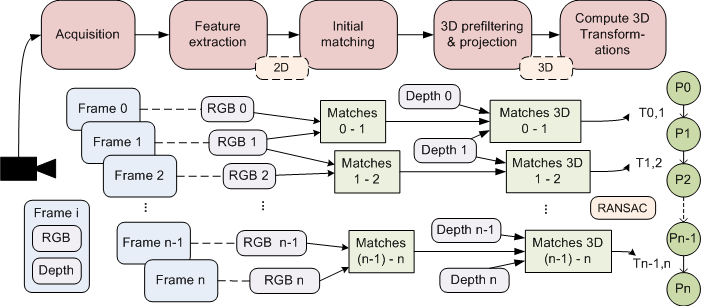
\includegraphics[width=1.0\textwidth]{figures/overview_rgb_depth}
\caption{Overview of how the RGB and depth input data can be used in order to produce the sequence of 3D transformations.}
\end{figure}

\chapter{Building a map}
\label{chap:map}

In the previous chapter, we saw how to determine a rigid transformation between a couple of frames. From each single transformation, an estimation of the poses of the camera can be computed. Now we can combine them to follow a sequence of frames. Each pose is then inserted into the graph by converting its representation from the camera matrix into a graph node. From the loop closures, new constraints can be inserted in the graph. The graph can then be optimized to globally reduce the error, and the poses updated according to the new vertices given by the graph after optimization.

\section{Estimating the poses}

Knowing the initial pose, the first step is to determine an estimation of any pose after a succession of transformations.

Considering a finite sequence of frames $[frame_0 ; frame_N]$, let~$P_k$ be the pose at rank $k \in [0;N]$, defined by a 4x4 matrix (6 Degrees-of-Freedom, 3 axis of rotation and translation, with homogeneous coordinates). For~$i>0$, we have the transformation~$T_{i_{-1},i}$ that binds the position~$P_{i-1}$ to the position~$P_i$. If~$P_0$ determines the initial position, we can then compute the position~$P_i$  by combining all the transformations like:

\begin{equation}
P_k = \prod_{i=k}^1{T_{i_{-1},i}} \: P_0
\label{eqn:pose_estimation}
\end{equation}

Note that, as the matrix product is not commutative, it is essential to follow the correct order when multiplying the matrices. For example, for the pose~$P_3$ we would have:

\[
P_3 = T_{2,3} \: T_{1,2} \: T_{0,1} \: P_0
\]

As an arbitrary choice, we can define the initial position to be at the origin of the coordinate system, ie the identity matrix~$I_4$.

\[
P_0 = I_4 = \left[ \begin{array}{cccc}
1 & 0 & 0 & 0 \\
0 & 1 & 0 & 0 \\
0 & 0 & 1 & 0 \\
0 & 0 & 0 & 1 \end{array} \right] 
\]

\section{Initializing the graph}

The equation \ref{eqn:pose_estimation} gives an estimation of the pose that can be inserted into the $g^2o$ graph.

The video sequence can lead to an important number of poses, especially if the robot slows down, or even stops. Inserting a node for each transformation would not be very efficient, as the same pose would be repeated in the graph. To distinguish these poses among all the others that can potentially be inserted in the graph, these poses are called the \emph{keyposes}. 

A simple solution is to define a keypose only after having achieved a move, with a given amplitude defined by a threshold. By cumulating the unitary moves between each couple of frame in the sequence, the creation of a new key pose is triggered once a given distance in translation or a given angle in rotation has been reached,  with respect to the last key pose. The thresholds are set by parameters, here 0.1m for the distance and 15\textdegree for the rotation (both values consider the 3 axis cumulated together). Another solution could be to compare the points of interests between the frames and trigger the creation of a new keypose when the number of points in common falls below a given threshold, but it is not given that the absolute number of points is representative enough to describe the amplitude of the move.

For each keypose, a node is inserted in the graph with an edge linking the new keypose with the previous one. A standard edge represents the rigid transformation between the two keyposes. Between each keypose, they may be a more than a couple of frames. To compute the corresponding transformation, the resulting matrix is found by multiplying the matrices of each couple of frames.

\section{Loop closures}

The next step is to insert additional constraints into the graph with the loop closure detection. Each time a loop closure is triggered between two keyposes, a new edge is inserted into the graph. To detect a loop closure, it is necessary to compare recent frames with previous ones. The naive approach would be to compare the current frame with all the previous frames. Generally, this is not realistic for reasons of performance, as the time necessary for the current frame would grow exponentially. This would be an issue if the matching verification is time consuming, or if the features of the past frames have to be recomputed each time. However, a preliminar check exclusively done on the RGB data, for example with color histograms, could be used to discard most of the negative candidates. Then, a more accurate verification with features could be done on the remaining candidates.

Without making any assumption of the past frames, the first idea would then be to define a window with a fixed size of n frames in the past. The most naive way is to select these frames randomly without any criterion.

Another approach would be to select the past frames that are more likely to match with the current frame. One solution could be to give a higher priority to the oldest frames. This could be done by defining a probability density function that would result in a higher probability for the oldest frames. Another approach would also involve a knowledge of the context of the frames, in terms of features, or in terms of estimated position.

%[TODO - for example, curves representing the probability to check a loop closure. Case linear, quadratic, threshold... ]
%[TODO - explain sliding window ]

\section{Optimizing the graph}

Once the graph has been initialized with the poses and the constraints from the loop closures, it can be optimized. Various methods are available in $g^2o$, for the optimization process and the solving problem. The method used here is Levenberg-Marquardt with a linear Cholmod solver. The optimization is done with a predefined number of steps. Once the graph has been optimized, the vertices are corrected and the new estimations of the camera poses can be extracted. The inverse operation is done to convert the information from the graph vertices to 4x4 matrices.

In $g^2o$ there is a tool (g2oviewer) allowing the visualization of the graph.

\begin{figure}[H]
\centering$
 \begin{array}{ccc}
 \includegraphics[width=0.3\textwidth]{pictures/graph4_base} &
 \includegraphics[width=0.3\textwidth]{pictures/graph4_initial_guess} &
 \includegraphics[width=0.3\textwidth]{pictures/graph4_optimized}
 \end{array}$
\caption{Graph with 4 rooms: non optimized - initial guess - after 10 iterations}
\end{figure}

\section{Scene reconstruction}

Finally, once the camera poses are determined with a good belief, the reconstruction of the scene can be performed. From each couple of RGB and depth data, a 3D point cloud can be generated providing the colour information for each point, but they still have to be put together. This process is called the point cloud \emph{registration}. Once the relative camera positions are known, one simple method is to transform each point cloud by reprojecting all its points according to the corresponding camera position, and concatenate together all the transformed point clouds.

This method remains simple, but the major issues are that it leads to duplicate points, and it does not take variances of illumination into account. The point cloud is not necessarily the best representation of the scene. Another solution would be to use some \emph{surfels} as done in the work of Henry~\cite{Henry_RGBD_2010}, but this would require some intensive processing and is out of the scope of this work.

\section{Summary}

We presented how the poses can be estimated, first by cumulating each transformation between a couple of frames. Through the use of a pose graph and the loop closures, their positions can be corrected over time. Finally, the map can be built through a scene reconstruction, by registration of the point clouds with the given positions of the cameras.

\chapter{Experiments}
\label{chap:experiments}

Now that the main aspects have been studied (feature extraction and matching, graph optimization, reconstruction), a software was developed, which goal is to acquire data from the Kinect, compute the 6~Degrees-of-Freedom camera poses representing the trajectory and orientation of the robot, and produce a 3D map. In order to repeat the experiments with different parameters, the data is saved and the program is able to replay a given sequence from a list of RGB-D files. The following sections describes how the input data was acquired and how the output is generated. The next sections present the maps obtained from different datasets, first from KTH, at different scales (1 room, 2 and 4 rooms with corridor). The last section shows the results obtained with data from other universities. 

\begin{figure}[h!]
\begin{center}
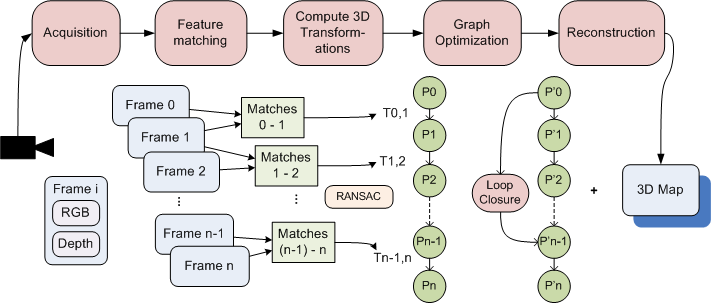
\includegraphics[width=1.0\textwidth]{figures/overview}
\caption{Overview of the system}
\end{center}
\end{figure}

\clearpage

\section{Data acquisition}

Two types of experiments were conducted: online, by moving the Kinect sensor by hand, and offline with the help of the robot in the \glsreset{CVAP}\gls{CVAP} at KTH. Experiments were carried out on a Pioneer III wheeled robot, Dora the explorer, with the Kinect camera mounted at 1.4 m above the floor and Hokuyo URG laser scanner. Each frame saved by the Kinect leads to a couple of RGB and Depth files taken at the same time. Additionally, the data from the laser scans and the odometry were saved. The acquisition of the data by the robot is not part of the program built in this work, this was done with the tools developed at \gls{CVAP}.

\begin{figure}[h]
 \begin{center}
 \includegraphics[width=0.8\textwidth]{pictures/Dora_7587}
 \end{center}
\caption{Dora the explorer}
\end{figure}

At KTH, the main dataset took place in environment with 4 different rooms connected by a corridor, resulting in 6474 frames (RGB-D datafiles) with several possibilities of loop closures. 

\begin{figure}[H]
\centering
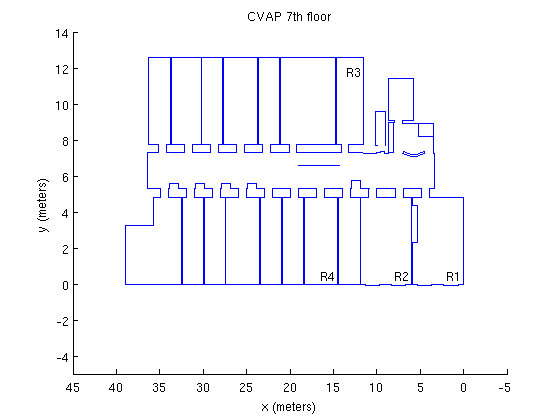
\includegraphics[width=1\textwidth]{figures/cvap_7th}
\caption{Reference map of the environment explored at CVAP. The visited rooms are labelled.}
\end{figure}

Other universities participating on common projects could provide data with a similar robot. This allowed to test the system with external data. We used the data provided by the universities of Birmingham and Ljubljana.

\begin{table}[H]
 \begin{center}
  \begin{tabular}{llcc}
  \hline
  University & Dataset & Rooms & Frames \\
  \hline
  KTH & 7th floor & 1 & 3082 \\
  KTH & 7th floor & 2 & 2697 \\
  KTH & 7th floor & 4 & 6474 \\
  Birmingham & Lab3 & 1 & 1342 \\
  Birmingham & Robot Lab & 1 & 2878 \\
  Ljubljana & Office1 & 1 & 2088 \\
  %TODO Office23 fails
  \hline
  \end{tabular}
 \end{center}
 \caption{Origin and size of the different datasets. Note that the KTH set of 1 room contains more frames than for 2 rooms, this is due to the robot moving at a slower speed.}
\end{table}

\clearpage

\section{Data output}

The result are the positions of the cameras, and the map represented by a point cloud. For reasons of performance, it is necessary to control the memory storage by limitating to the size of the final point cloud. Theorically, each point cloud can be composed of $640\times480 = 307,200$ points. Practically, the effective number of points is lower, as the depth information is not available for each point (due mainly to the range limit and to the occlusions considering the difference of point of view between the IR and RGB sensors). A standard point cloud is composed of about 200,000 points. For each pixel, 24 bits are used for the positions (x,y,z) and 24 bits for the colors R,G,B ($3\times8$ bits), padded to 8 bytes for alignment in memory. Therefore, a colored cloud point occupies around $200k\times8$ = 1.6MB in memory. For a scope of visualization, it is reasonable to reduce the amount of information. Each point cloud is first subsampled simply by removing points taken randomly with a given probability (according to a fixed ratio, set as a parameter depending on the global size of the scene).

Generally, only one output file is produced but this could still lead to a big file in case of a large map. In this case, the total number of points can still be relatively important and a too high rate of subsampling would lead to a map of low quality. By setting a threshold for the size of the final point cloud file, it can be splitted in several subfiles each time the threshold is reached during the reconstruction of the global map. The result is then divided in different files. This allows to keep a low subsampling rate, and still to visualize a portion of the global scene with a good definition. For the visualization of the point clouds, the standard viewer provided in \gls{PCL} is used.

\section{Software implementation}

The code is available as an open source project\footnote{\url{http://code.google.com/p/kth-rgbd/}}. It is released with a LGPL v3 license.
The program does the following tasks:
\begin{itemize}
\item Acquire RGB-D data from the Kinect
\item Perform features extraction and matching on a sequence of frames and compute the relative transformations with \gls{RANSAC}
\item Compute the positions of the camera poses and translate them into graph nodes and edges
\item Compute the loop closures and insert the corresponding edges into the graph
\item Optimize the graph and extract the updated camera poses
\item Reconstruct the global scene by generating a point cloud datafile (*.pcd)
\end{itemize}

The number of dependencies has been limited as much as possible, using preferably open-source libraries. At the difference with the RGBD-6D-SLAM project~\cite{engelhard11euron-workshop} it is not based on \gls{ROS} framework, but only \gls{PCL} for the reconstruction at the final step. The main dependencies are the following:
\begin{itemize}
\item g2o: the graph optimization
\item OpenNI: to acquire the Kinect data
\item OpenCV: open source library used to visualize the intermediate results with bitmaps (frame matching) and compute the \gls {SURF} features
\item SIFT Library by Rob Hess~\cite{hess_sift}: for the \gls{SIFT} extraction and initial matching
\item Eigen3: for the geometric support with transformations and matrices
\item Point Cloud Libary~\cite{Rusu_ICRA2011_PCL}, standalone distribution (cminpack, Flann, Eigen3, OpenNI): for the transformations and the export to point cloud datafiles
\item Boost: support library, used here to access the filesystem
\end{itemize}

%$g^2o$ provides the class SE3Quat which implies the transformation of the rotational part of the matrix into a quaternion. Compared to Euler angles, the advantage of the quaternion is a more compact representation (4 terms instead of 9), a more efficient for the numerical computations and it allows to avoid some particular cases like the gimbal locks. In this work, we still keep a standard representation with a 4x4 matrix for the transformation (rotation \& translation) until the interaction with $g^2o$.

\clearpage

\section{Map CVAP, one room}

\subsection{Without loop closures}

\begin{figure}[H]
\centering
\includegraphics[width=0.8\textwidth]{pictures/room1_initial}
\caption{Map with 1 room, without graph optimization. Note how the corner of the table and the chair appears to be doubled.}
\end{figure}

\subsection{With loop closure}
This map is built from a sequence containing one room, the graph is optimized with one loop closure, which is triggered after having gone through the room and back to a position close to the initial position. 

\begin{figure}[H]
\centering
\includegraphics[width=0.8\textwidth]{pictures/room1_1}
\caption{Map with 1 room, optimized with one loop closure. Note how the corner of the table and the chair are now correctly "merged" compared to the previous figure.}
\end{figure}

\section{Map CVAP, two rooms and corridor}

\begin{figure}[H]
\centering$
 \begin{array}{c}
 \includegraphics[width=0.8\textwidth]{pictures/room2_1}\\
 \includegraphics[width=0.8\textwidth]{pictures/room2_2}
 \end{array}$
\caption{Map with 2 rooms, optimized with two loop closures}
\end{figure}

\section{Map CVAP, four rooms and corridor}

\subsection{Without loop closure}

\begin{figure}[H]
\centering$
 \begin{array}{c}
 \includegraphics[width=0.8\textwidth]{pictures/room4_new_init1}\\
 \includegraphics[width=0.8\textwidth]{pictures/room4_new_init2}
 \end{array}$
\caption{Map with 4 rooms and corridor, not optimized. The main problem can be seen in the living room, see the double chair.}
\end{figure}

\begin{figure}[H]
\centering$
 \begin{array}{c}
 \subfloat[]{\label{fig:poses_4r_1_1} 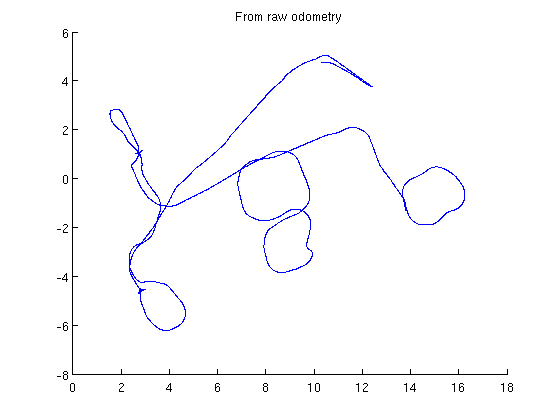
\includegraphics[width=0.6\textwidth]{figures/poses_4r_odometry_raw}} \\
 \subfloat[]{\label{fig:poses_4r_1_2} 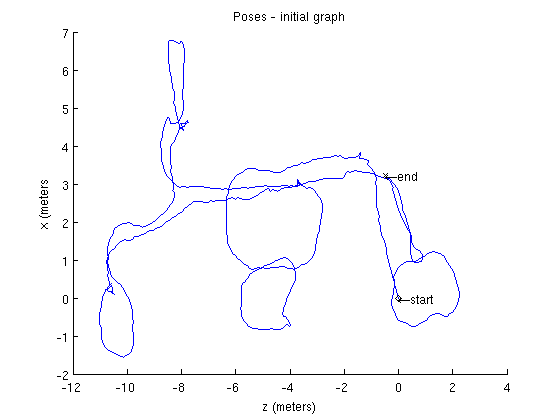
\includegraphics[width=0.6\textwidth]{figures/poses_4r_initial}}
 \end{array}$
\caption{Estimation of the poses - \protect\subref{fig:poses_4r_1_1} From standard odometry, raw data. Note the drift, as the start and end points should be pretty close. \protect\subref{fig:poses_4r_1_2} With this system, initial graph. }
\end{figure}

\subsection{With loop closure}

\begin{figure}[H]
\centering$
 \begin{array}{c}
 \includegraphics[width=0.8\textwidth]{pictures/room4_new_optim1}\\
 \includegraphics[width=0.8\textwidth]{pictures/room4_new_optim2}
 \end{array}$
\caption{Map with 4 rooms and corridor, optimized with several loop closures. It looks a bit worse than the initial one. The double chair corrected in the living room but corridor and room alignments are worse.}
\end{figure}

\begin{figure}[H]
\centering$
 \begin{array}{c}
 \subfloat[]{\label{fig:poses_4r_2_1} 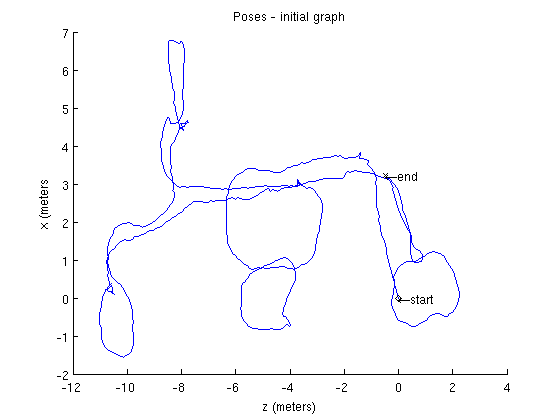
\includegraphics[width=0.6\textwidth]{figures/poses_4r_initial}} \\
 \subfloat[]{\label{fig:poses_4r_2_2} 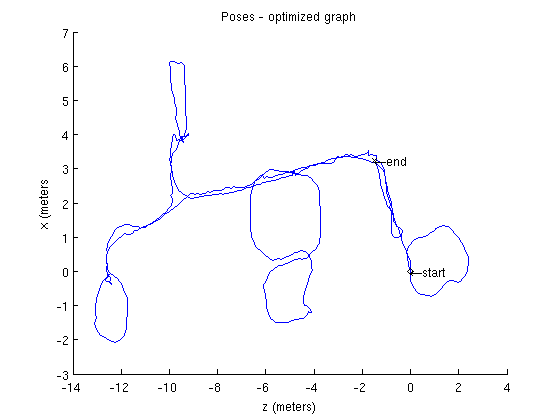
\includegraphics[width=0.6\textwidth]{figures/poses_4r_optimized}}
 \end{array}$
\caption{Estimation of the poses - \protect\subref{fig:poses_4r_2_1} With the initial graph.  \protect\subref{fig:poses_4r_2_2} With the optimized graph. There is a slight variation. }
\end{figure}

\begin{figure}[H]
\centering
\includegraphics[width=1\textwidth]{figures/cvap_7th_4r_sift}
\caption{Trajectory overlayed on the reference map of the 7th floor, with SIFT features.}
\end{figure}

\begin{figure}[H]
\centering
\includegraphics[width=1\textwidth]{figures/cvap_7th_4r_surf}
\caption{Trajectory overlayed on the reference map of the 7th floor, with SURF features.}
\end{figure}

\begin{figure}[H]
\centering$
 \begin{array}{c}
 \includegraphics[width=1.0\textwidth]{figures/drift_y_sift} \\
 \includegraphics[width=1.0\textwidth]{figures/drift_y_surf}
 \end{array}$
\caption{Analysis of the vertical drift. Coordinate Y has been rescaled to origin. Considering the camera is fixed on a support, the value should stay close to zero.}
\end{figure}

\clearpage
\section{Map from other universities}

\begin{figure}[H]
\centering$
 \begin{array}{c}
 \includegraphics[width=0.5\textwidth]{pictures/bham_lab3_1}
 \includegraphics[width=0.5\textwidth]{pictures/bham_lab3_2}
 \end{array}$
\caption{Birmingham Lab3}
\end{figure}

%\begin{figure}[H]
%\centering$
%\begin{array}{c}
%\includegraphics[width=0.5\textwidth]{pictures/bham_robotlab_1}
%\includegraphics[width=0.5\textwidth]{pictures/bham_robotlab_2}
%\end{array}$
%\caption{Birmingham Robotic Lab}
%\end{figure}

\begin{figure}[H]
\centering
\includegraphics[width=0.8\textwidth]{pictures/bham}
\caption{Birmingham office}
\end{figure}

\begin{figure}[H]
\centering$
 \begin{array}{cc}
 \subfloat[]{\label{fig:ljub1_1} \includegraphics[width=0.4\textwidth]{pictures/ljub_office1}} &
 \subfloat[]{\label{fig:ljub1_2} \includegraphics[width=0.4\textwidth]{pictures/ljub_office1_feature}}
 \end{array}$
\caption{Ljubljana office1 - \protect\subref{fig:ljub1_1} Map without closure loop. \protect\subref{fig:ljub1_2} Not enough features could be extracted at this point.}
\end{figure}


\begin{figure}[H]
\centering
\includegraphics[width=0.8\textwidth]{pictures/ljub_office2and3}
\caption{Ljubljana office2 - map without closure loop}
\end{figure}

\section{Summary}

These results show that 3D maps can be built with this system and illustrate the interest of the loop closure to get a good correction. But it does not necessarily  give the optimal result, and there can be a drift as soon as the size of the map grows. Here, the maps with 4 rooms show some noticeable errors. This also shows that the process can be interrupted as soon as there are not enough visual features to detect a valid transformation.

%In terms of performance, we compared SIFT and SURF on the largest dataset.
%
%\begin{table}[H]
% \begin{center}
%  \begin{tabular}{llcc|cc}
%  \hline
%  University & Dataset & Rooms & Frames & SIFT & SURF \\
%  \hline
%  KTH & 7th floor & 4 & 6474 & 2h24mn & 0h54mn \\
%
%  \hline
%  \end{tabular}
% \end{center}
% \caption{Performance using SIFT and SURF.}
%\end{table}



\chapter{Conclusions and Future Works}
\label{chap:conclusion}

This work gave a good insight into the general problem \gls{SLAM}, and more specifically about \gls{VSLAM} with feature extraction and matching. The approach can be described in the following steps:
\begin{enumerate}
\item Feature extraction: \gls{SIFT}/\gls{SURF} extraction in 2D
\item Feature matching: kd-tree on the feature space, using the depth for a preselection of the features
\item Transformation: \gls{RANSAC} on the projected points in 3D
\item Graph optimization: based on the $g^2o$ framework
\item Loop Closures: add some constraints in the graph by detecting scenes already seen in the past
\item Scene reconstruction: registrate the points clouds accordingly to the estimation of the keyposes, and concatenate them to build the global map.
\end{enumerate}

Given this, it is now possible to imagine some improvements of the current work, both in terms of quality of the results and overall performance.

\section{Quality improvements}

\begin{itemize}
\item Finding a better transformation: the \gls{RANSAC} method gives a rigid transformation that is not necessarily the best. The parameters may be tuned in a more efficient way to give more accurate results, or using a variant like MLESAC \cite{TorrZ00}. The tuning also concerns the initial matching done with the \gls{SIFT}/\gls{SURF} features. The \gls{ICP} \cite{zhang_92_icp} method should give a refined solution. The output of the \gls{RANSAC} loop could be used as an initial guess for \gls{ICP}. 
\item Graph optimization: it could be improved by defining more accurately the optimization problem and studying the most appropriate method (possibly with~$g^2o$ by deriving new classes and defining appropriate error functions), and also by working with different scales (hierarchical levels for bigger maps). New criterions could be defined for loop closures, by introducing some knowledge about the past frames (features or estimated position more likely to give a loop closure with the current frame) or by detecting a portion of scene that does not give a valid transformation in the current system.
\item Additional sensors: in this work, the only sensor used was the Kinect providing RGB-D data. One possibility would be to use others sensors and combine them to get a better result, especially when the transformations computed by the method presented in this work are less reliable.
\end{itemize}

\section{Performance improvements}

Currently, most of the time is passed on the feature extraction. Here are a few alternatives :
\begin{itemize}
\item GPU implementation: a feature extraction optimized for the hardware of the graphic cards would dramatically lower the computational time to enable real-time applications. Various GPU implementations exist for both SIFT and SURF, that would certainly lead to a feature extraction under 100ms on the current platform. In addition, some solutions take advantage of the parallel computing on specific platforms, such as CUDA\texttrademark{} for the NVIDIA graphic cards. The features extraction could then be performed in 15-20ms.
\item BRIEF: combined with a keypoint detector such as \gls{SURF} or \gls{SIFT}, the \gls{BRIEF} descriptors~\cite{Calonder10-brief} could give an interesting alternative, being more efficient to compute. However, this would imply to rewrite the matching code, by doing binary string comparison. See also the PhD thesis of Calonder~\cite{Calonder10_PhD}.
\item ICP: though the standard algorithm could increase the computational time, some efficient variations exist~\cite{Rusinkiewicz_2001}. 
\end{itemize}

\section{Other approach}

With the KinectFusion project, Microsoft presents a solution performing reconstruction without any feature, though it achieves real-time performance as demonstrated\footnote{KinectFusion: \url{http://www.youtube.com/watch?v=quGhaggn3cQ} (last access Nov 2011)} at SIGGRAPH~2011. The camera tracking is based on a GPU implementation of \gls{ICP} on the point clouds generated from the depth data. The related papers \cite{Izadi_2011_SIGGRAPH} \cite{Newcombe_2011_ISMAR} describe how an accurate dense reconstruction can be performed in real-time, which sounds promising in the future for many applications related to computer vision, not only mapping but also segmentation and object recognition.
